\documentclass[11pt]{report}
\usepackage{eso-pic,graphicx}
\usepackage[export]{adjustbox}
\usepackage{url}
\usepackage{amsmath}
\usepackage[top=2cm, bottom=2cm, outer=2cm, inner=2cm]{geometry}
\begin{document}
\AddToShipoutPictureBG*{
\includegraphics[width=\paperwidth,height=\paperheight]{images/bkgrnd}}
\begin{center}
\vspace*{2cm}
\textsf{\begin{Huge}
\textbf{ELP­718 ­ Telecom Software Laboratory \\
1st Semester, 2016-18 \\
Abhishek Mishra\\
03 Nov 2016, 5pm\\
Assignment-12}\\
\end{Huge}}
\vspace*{6cm}

\includegraphics[scale=0.12, center]{images/iitlogo}
\end{center}
\pagebreak
\tableofcontents
\vspace{5cm}
\pagebreak
\section{Introduction}
\vspace*{1cm}
This assignment aims to provide a better understanding of the following topics:\\
\begin{flushleft}
1. \textbf{Lex}\\
Lex helps write programs whose control flow is directed by instances of regular expressions in the input stream. It is well suited for editor-script type transformations and for segmenting input in preparation for a parsing routine.
\\
Lex source is a table of regular expressions and corresponding program fragments. The table is translated to a program which reads an input stream, copying it to an output stream and partitioning the input into strings which match the given expressions. As each such string is recognized the corresponding program fragment is executed. The recognition of the expressions is performed by a deterministic finite automaton generated by Lex. The program fragments written by the user are executed in the order in which the corresponding regular expressions occur in the input stream.
\end{flushleft}

\begin{flushleft}
2. \textbf{Yacc}\\
Computer program input generally has some structure; in fact, every computer program that does input can be thought of as defining an ``input language'' which it accepts. An input language may be as complex as a programming language, or as simple as a sequence of numbers. Unfortunately, usual input facilities are limited, difficult to use, and often are lax about checking their inputs for validity.\\
Yacc provides a general tool for describing the input to a computer program. The Yacc user specifies the structures of his input, together with code to be invoked as each such structure is recognized. Yacc turns such a specification into a subroutine that han- dles the input process; frequently, it is convenient and appropriate to have most of the flow of control in the user's application handled by this subroutine.
\end{flushleft}
\newpage
\section{Problem Statement}
Design a Database system for Bharti School which holds the details of the Student, Courses being float and the Students enrolled in those Courses.\\
The Relational tables required for this task are:\\
\begin{gather*}
\textbf{Student}(Stu\_id, Name, Gender);\\
\textbf{Course}(Course\_id, Course name, Instructor);\\
\textbf{Enroll}(Stu\_id, Course\_id);\\
\textbf{Grades}(Stu\_id, Course\_id, Grade);\\
\end{gather*}
	
\subsection{Assumptions}
The number of Courses being float are 8 only which are Signal Theory, Telecom Software Lab, Computer Networks, Telecom Technologies, Telecom Management System, Braodband Communication, Coding Theory, Digital Communication. \\
The Instructors are Prof. Subrat Kar, Prof. Ranjan Bose, Prof. Mahim Sagar, Prof. Shankar Prakriya.\\
A Student is allowed to enroll in atmost 4 Courses.\\
There is atleast a student in a Course.
\subsection{Part 1}
Design Database for given system using MySQL i.e. create one database and the relational tables described above. Also write a python code to populate the tables.\\
The generated table looks like this:\\
\begin{figure}[h!]
\centering
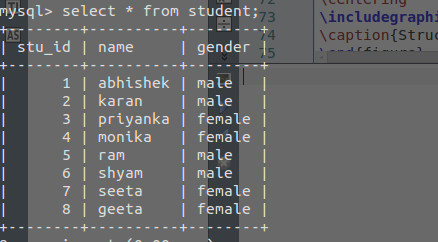
\includegraphics[scale=0.7]{images/part1stud}
\caption{Table Student}	
\end{figure}
\pagebreak
\begin{figure}[h!]
\centering
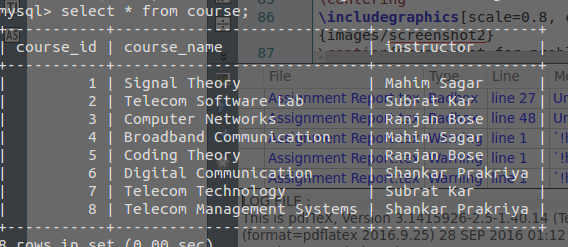
\includegraphics[scale=0.7]{images/part1course}
\caption{Table Course}	
\end{figure}
\pagebreak
\begin{figure}[h!]
\centering
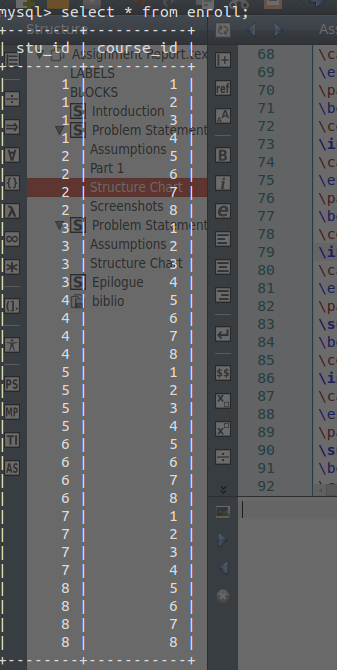
\includegraphics[scale=0.7]{images/part1enroll}
\caption{Table Enroll}	
\end{figure}
\pagebreak
\begin{figure}[h!]
\centering
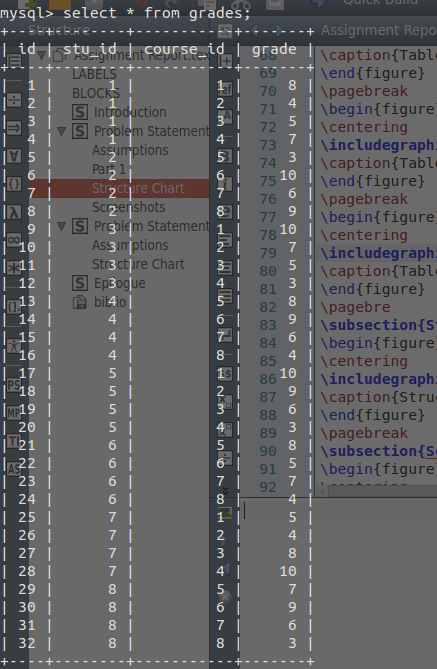
\includegraphics[scale=0.7]{images/part1grades}
\caption{Table Grades}	
\end{figure}
\pagebreak
\subsection{Part 2}
Write SQL query to find the names of those students who have enroll in both Coding theory and Telecom Management system.
\subsection{Part 3}
Write SQL query to find the names of those Students who have Scored an “A” in atleast one of the Subject taught by Prof. Subrat Kar.
\subsection{Part 4}
Write SQL query to find average grade for each of the course.
\subsection{Part 5}
Write SQL query to find the names of girl student who have topped in the course along with the course name.
\pagebreak
\subsection{Structure Chart}
\begin{figure}[h!]
\centering
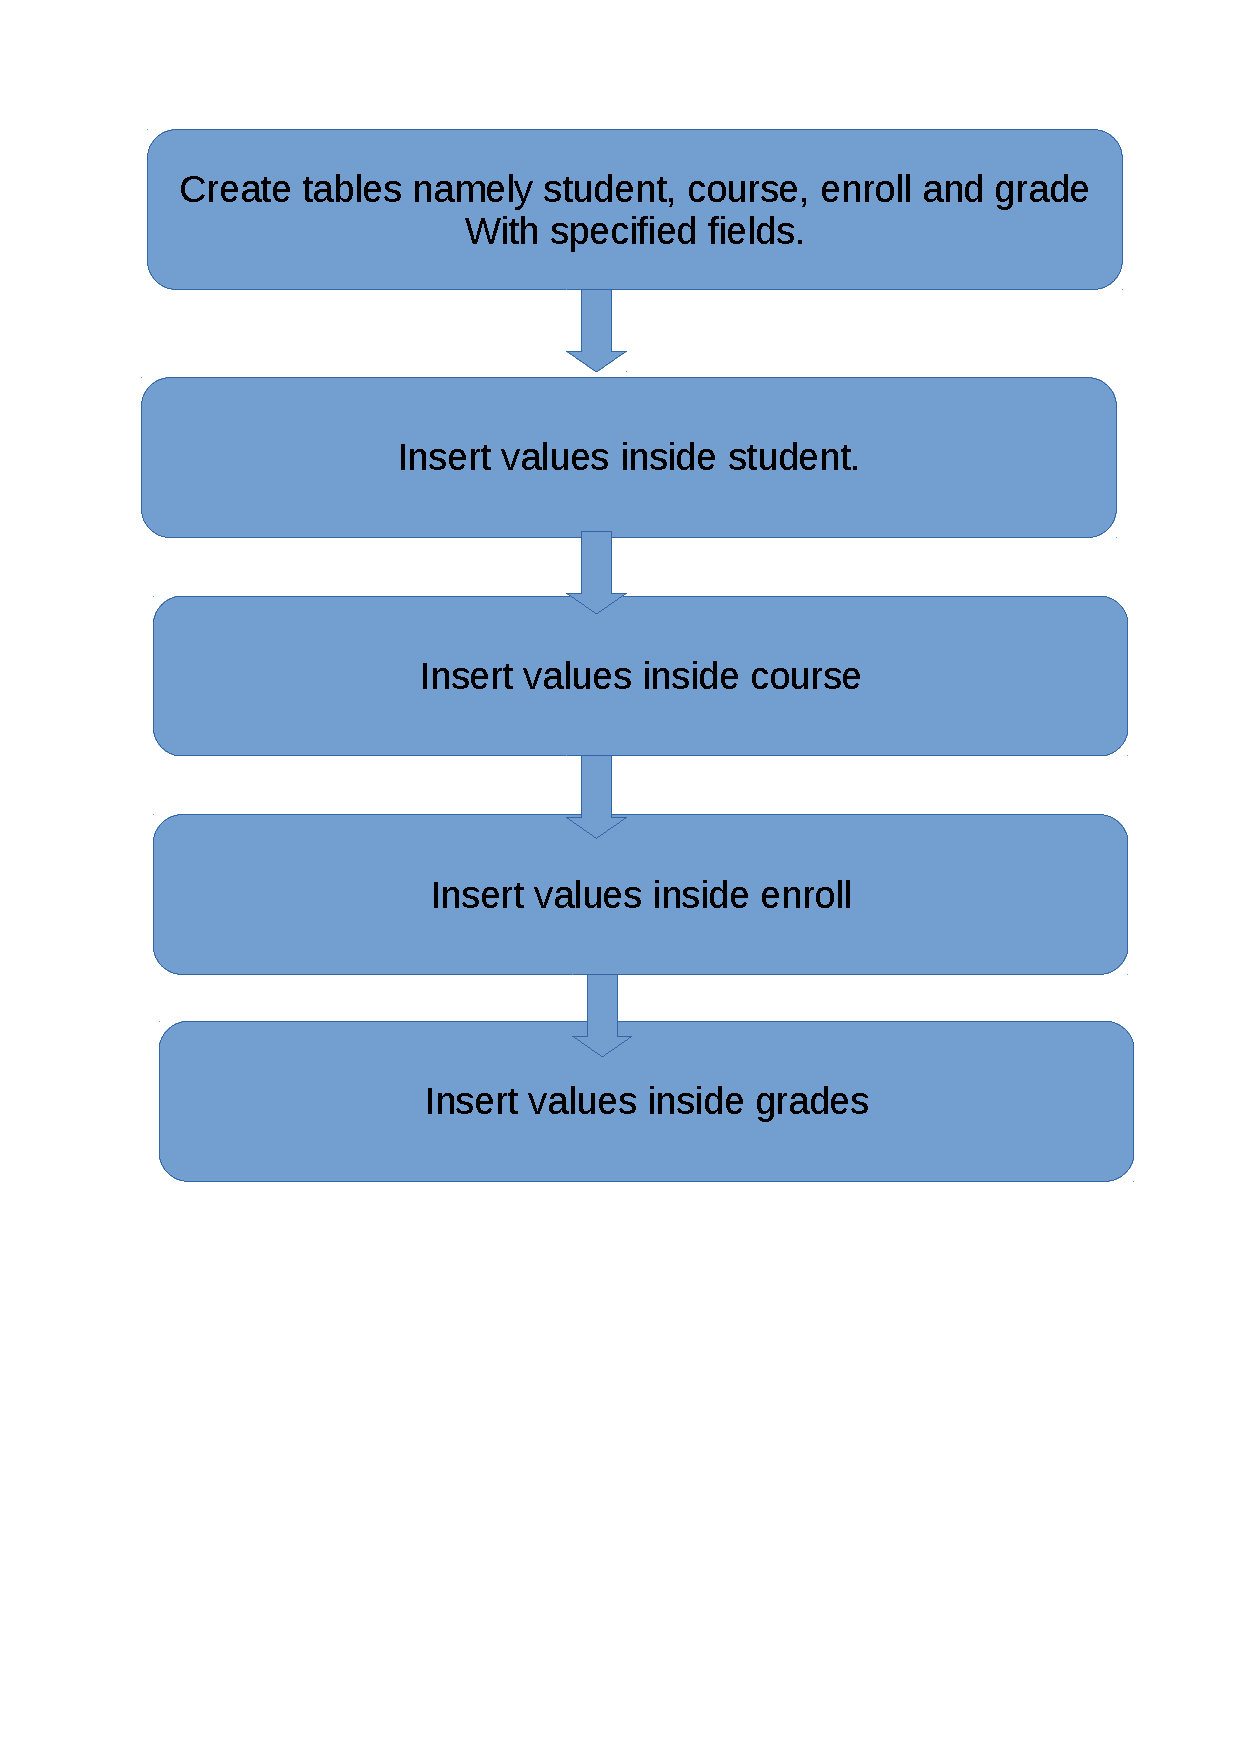
\includegraphics[scale=0.7]{images/sc1}
\caption{Structure chart for Part 1}	
\end{figure}
\pagebreak
\begin{figure}[h!]
\centering
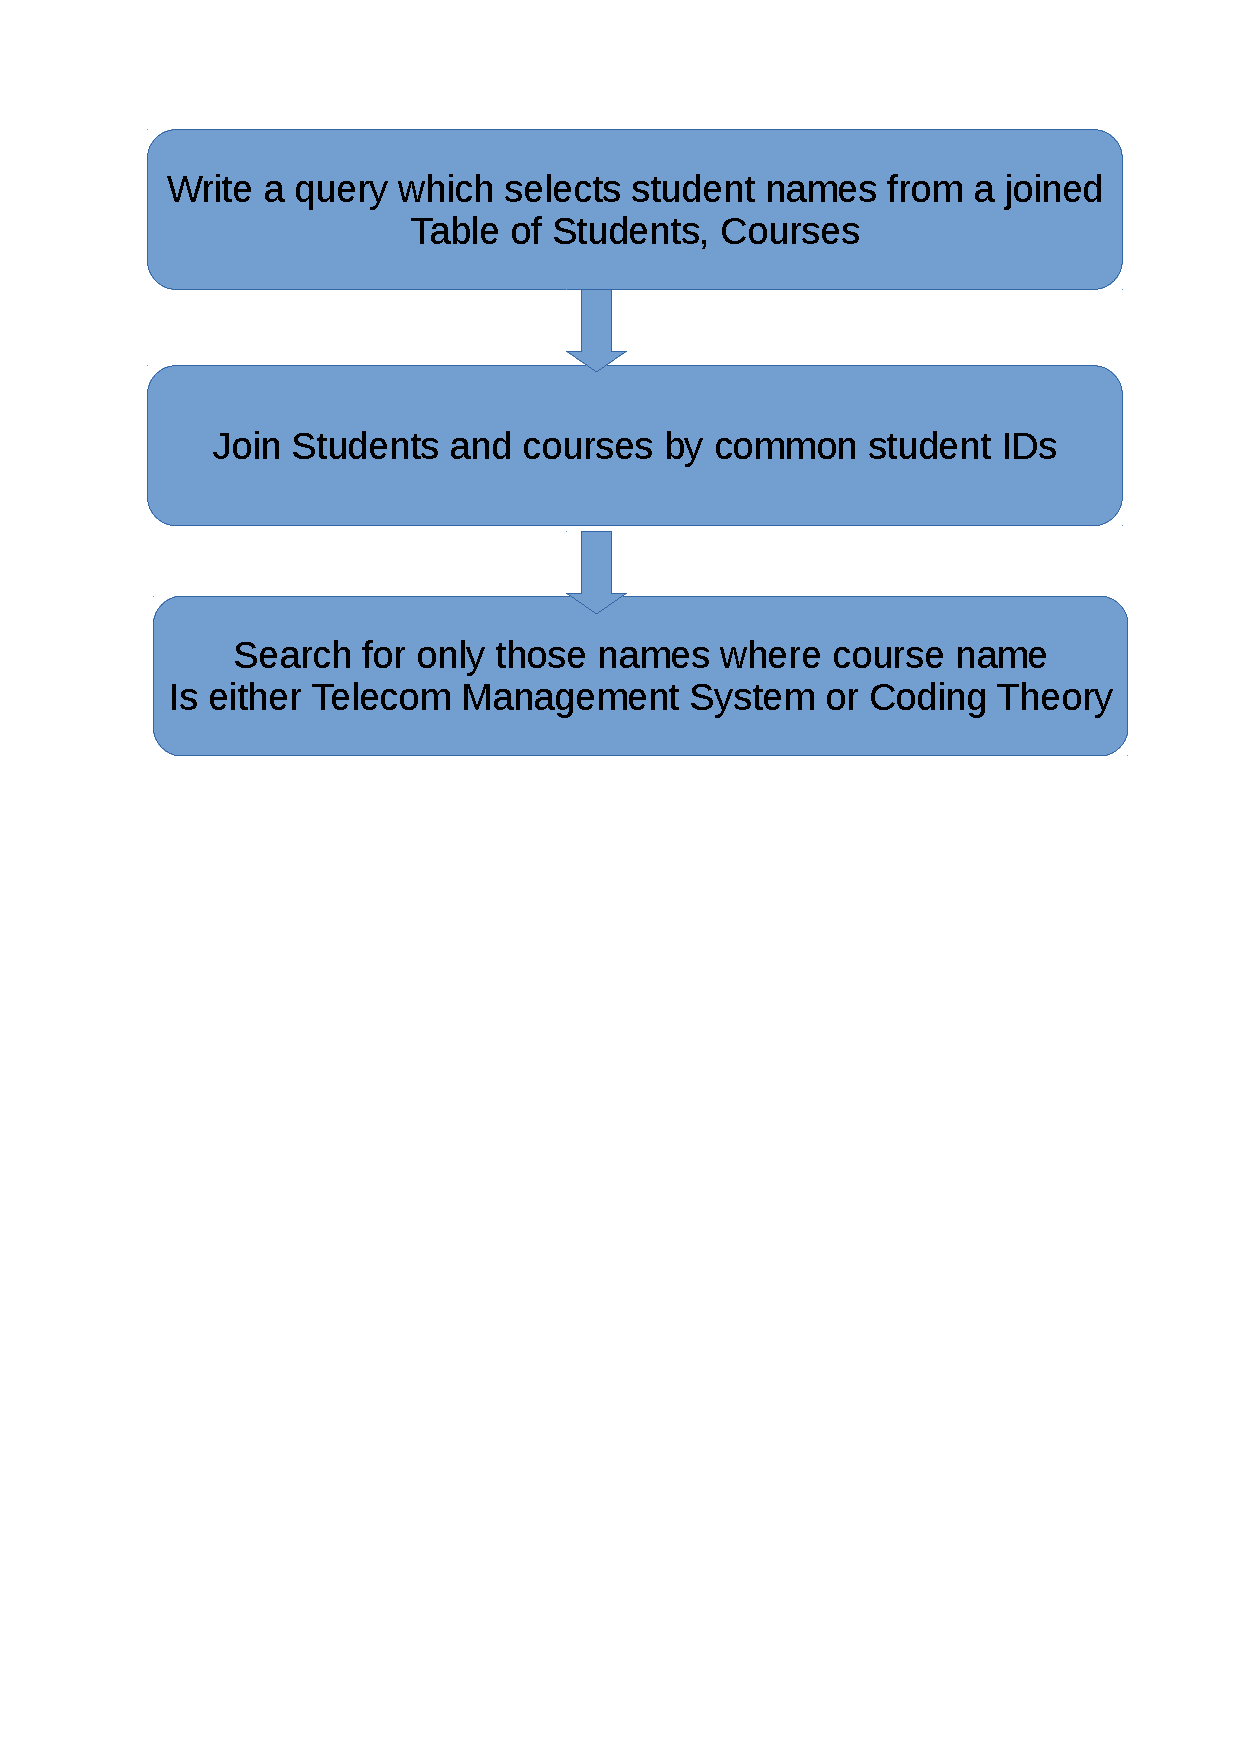
\includegraphics[scale=0.7]{images/sc2}
\caption{Structure chart for Part 2}	
\end{figure}
\pagebreak
\begin{figure}[h!]
\centering
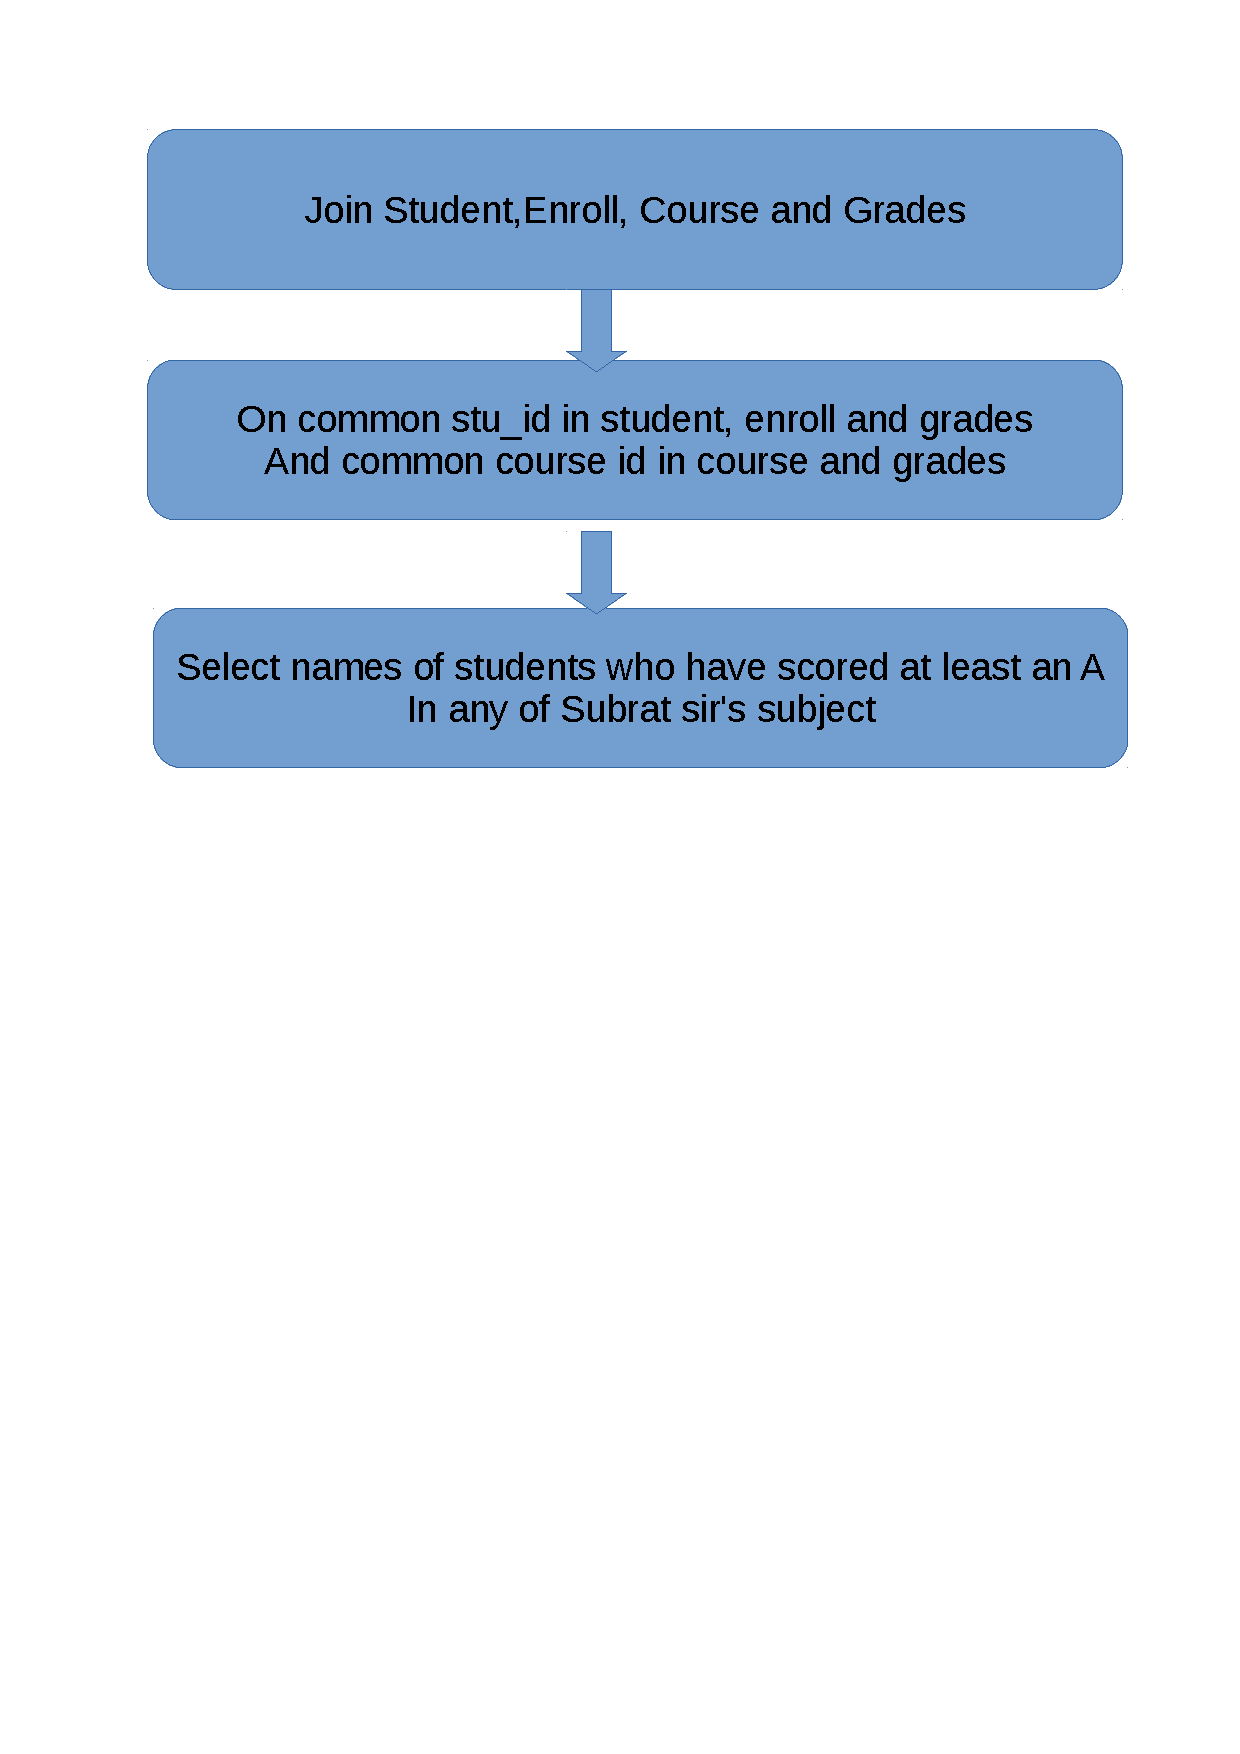
\includegraphics[scale=0.7]{images/sc3}
\caption{Structure chart for Part 3}	
\end{figure}
\pagebreak
\begin{figure}[h!]
\centering
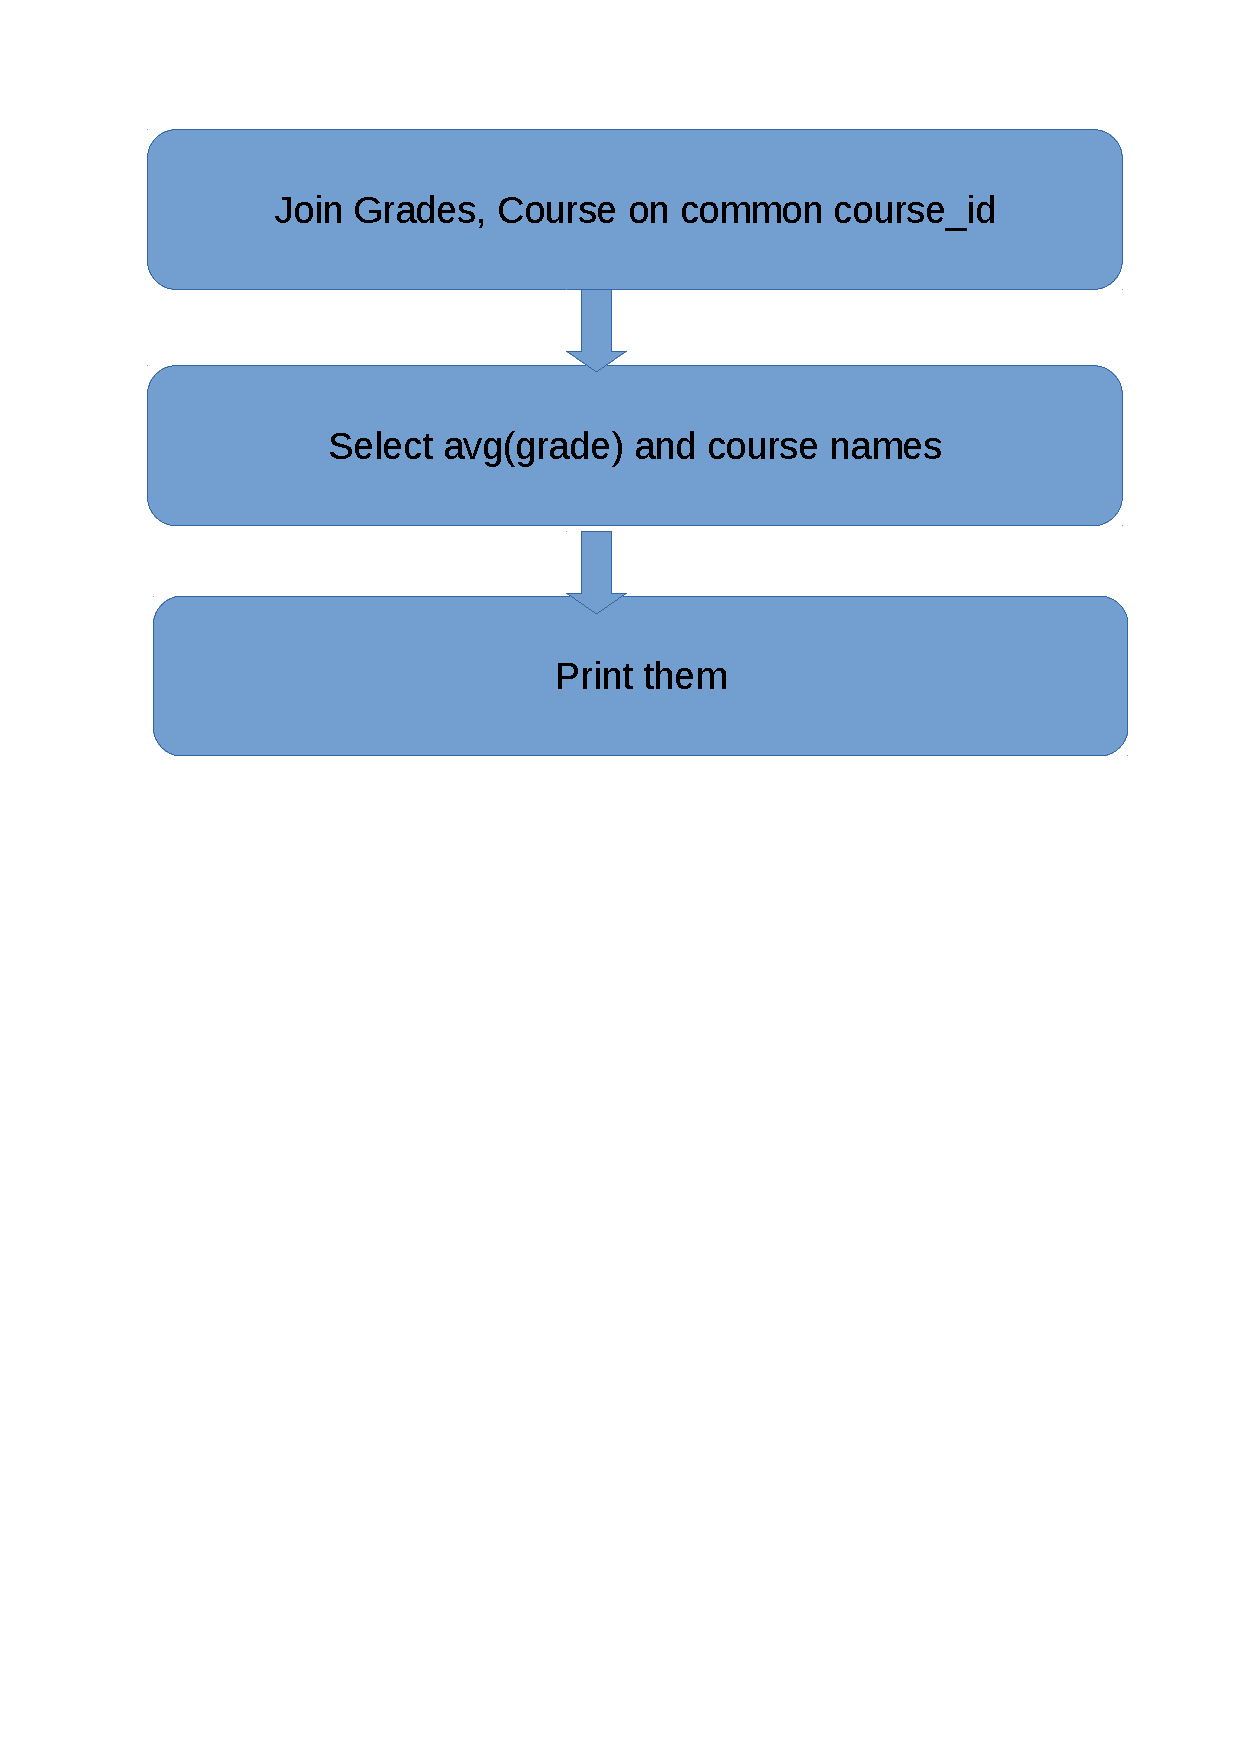
\includegraphics[scale=0.7]{images/sc4}
\caption{Structure chart for Part 4}	
\end{figure}
\pagebreak
\begin{figure}[h!]
\centering
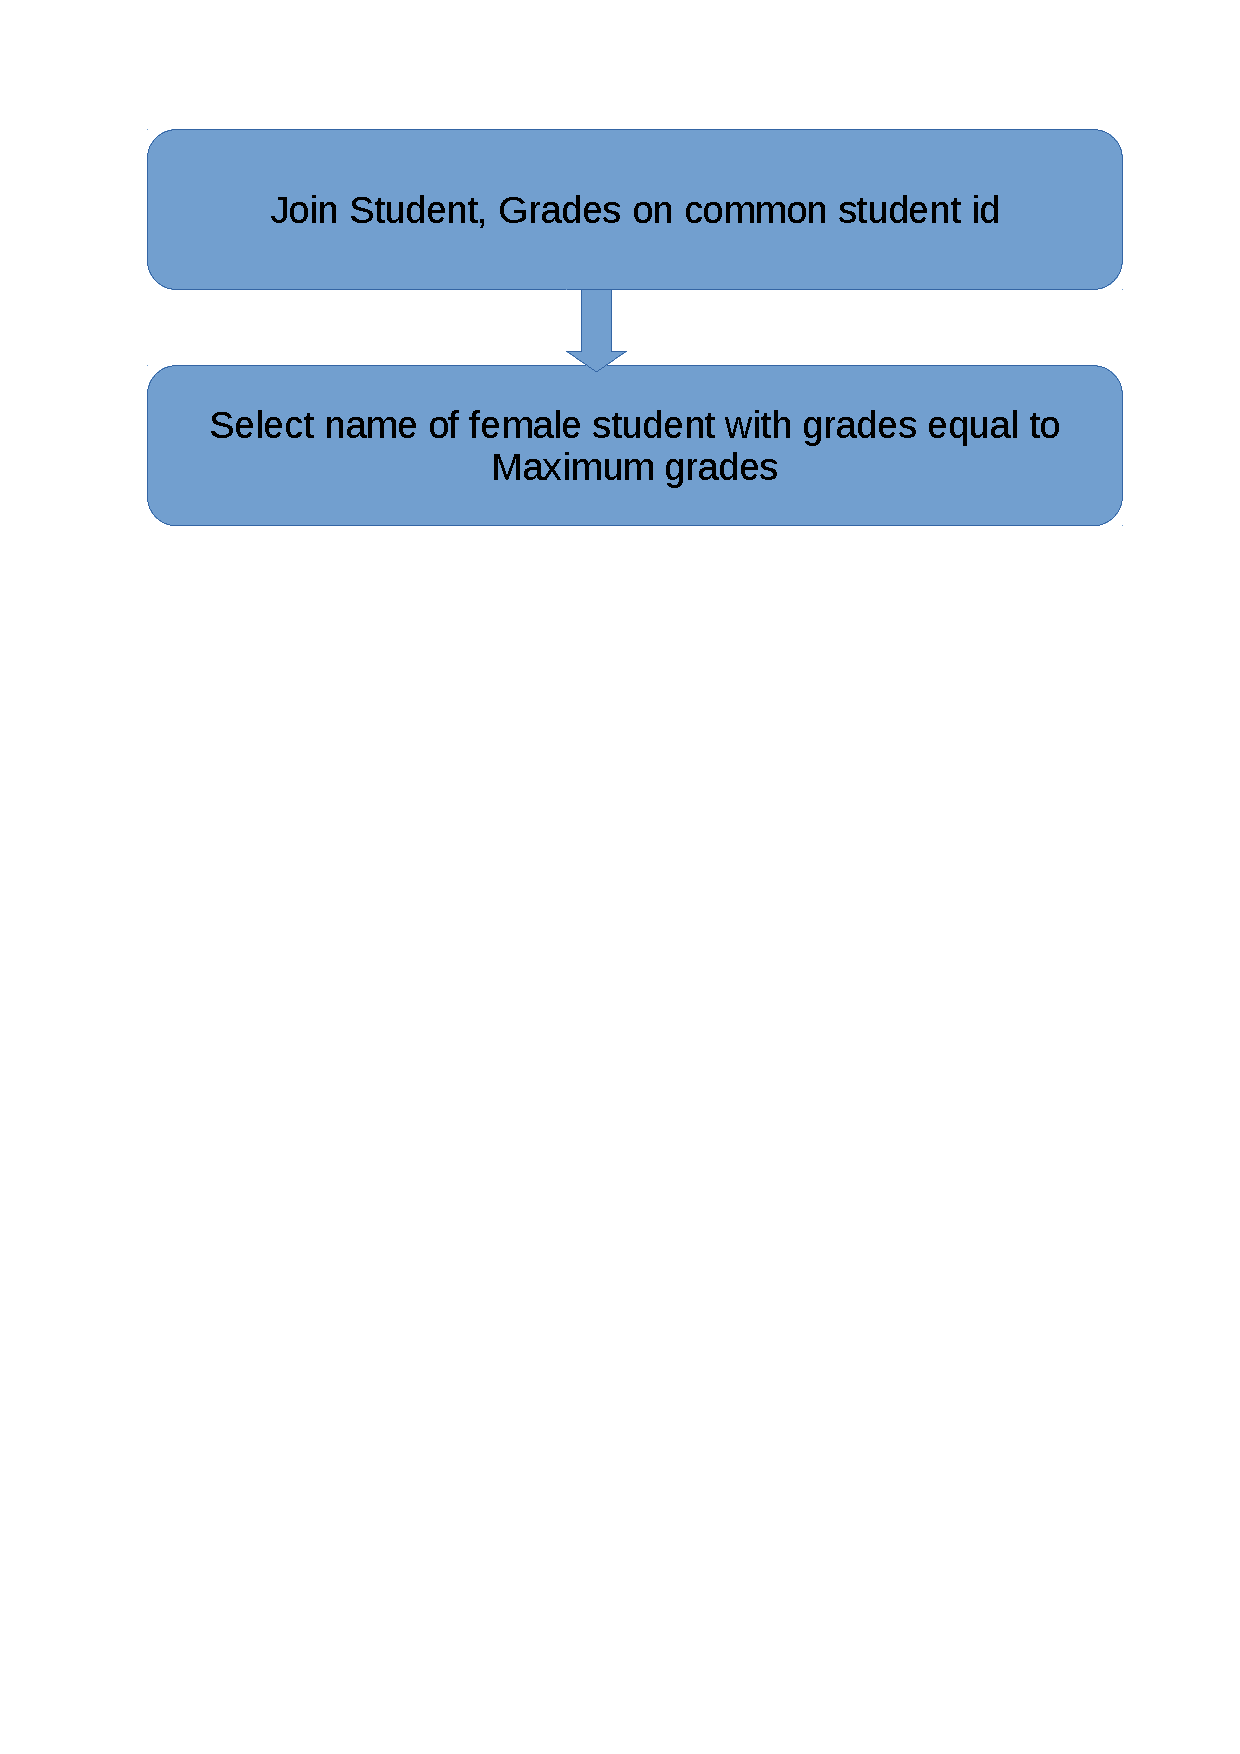
\includegraphics[scale=0.7]{images/sc5}
\caption{Structure chart for Part 5}	
\end{figure}
\pagebreak
\subsection{Screenshots}
\begin{figure}[h!]
\centering
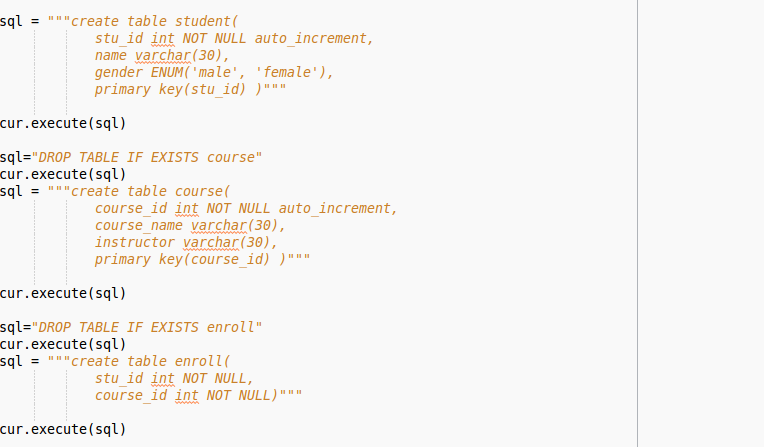
\includegraphics[scale=0.8, center]{images/screenshot1}
\caption{Screenshot for part 1}
\end{figure}
\pagebreak
\begin{figure}[h!]
\centering
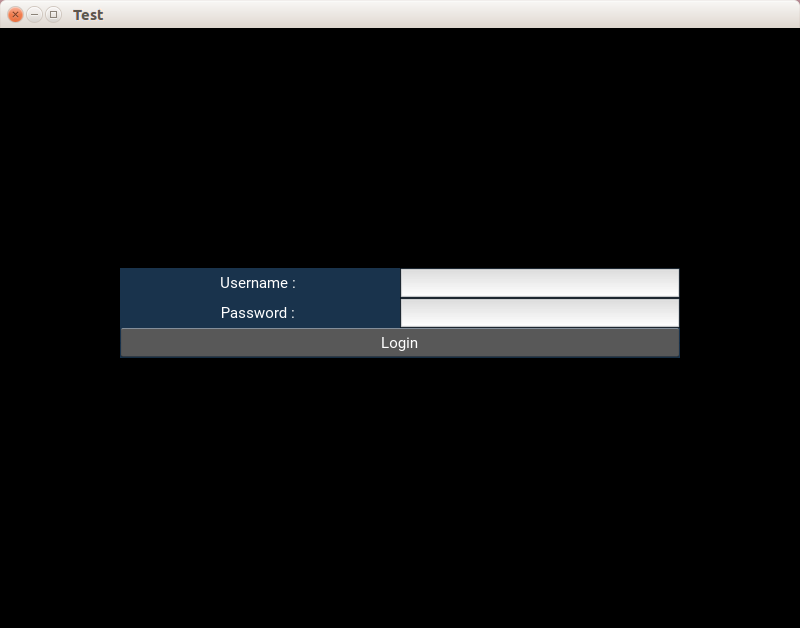
\includegraphics[scale=0.8, center]{images/screenshot2}
\caption{Screenshot for part 2}
\end{figure}
\pagebreak
\begin{figure}[h!]
\centering
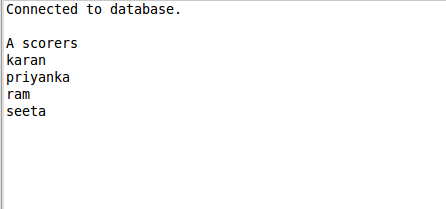
\includegraphics[scale=0.8, center]{images/screenshot3}
\caption{Screenshot for part 3}
\end{figure}
\pagebreak
\begin{figure}[h!]
\centering
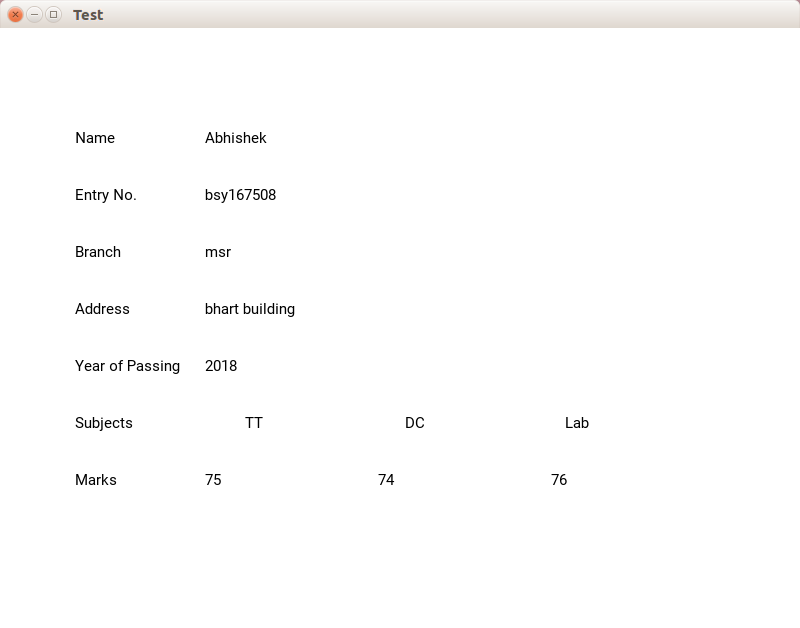
\includegraphics[scale=0.8, center]{images/screenshot4}
\caption{Screenshot for part 4}
\end{figure}
\pagebreak
\begin{figure}[h!]
\centering
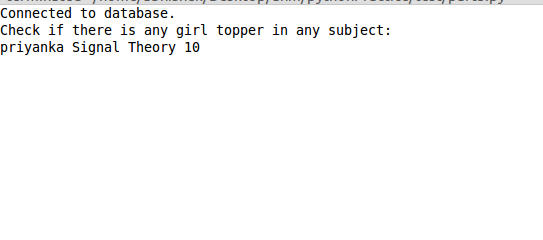
\includegraphics[scale=0.8, center]{images/screenshot5}
\caption{Screenshot for part 5}
\end{figure}
\pagebreak
\section{Epilogue}
This week's assignment tested our database management skills and our ability to form basic RDBMS relations and using them to execute our required tasks. 
\bibliography{biblio} 
\bibliographystyle{ieeetr}
\nocite{*}
\end{document}